% SPECIFIC OPTIONS:
%     eng:   Idioma inglés (por defecto)
%     esp:   Idioma español
%     por:   Idioma portugués
%     blind: Se compila la versión para revisores (se ocultan datos de los autores)

\documentclass[esp]{FCEFyN-class}
%
% Título de la publicación
\title{Theoretical and Experimental Studies of Metallic Hydrogen}

% Título corto para el encabezado (copiar el título principal si no resulta demasiado largo)
\shorttitle{}
       
% Autores
\author{R. Peal, S. Ferguson, AM. Penot, V. Dejean, B. Micah, MV. de Toro Sánchez}




% Datos de la publicación (serán definidas en la edición)



\addbibresource{biblio.bib}

% Iniciar documento
\begin{document}
% Introduzca aquí el resumen en español (o en portugués si utiliza la opción [por])
\resumen{
Hydrogen is the simplest, most abundant element in the universe. Though more familiar as a gas, below about 800 K and 400 GPa hydrogen becomes a molecular solid. It is predicted that at 400--500 GPa and below about 450 K, hydrogen will transition to a metal. Metallic Hydrogen (MH) is of significant scientific interest as investigating the behaviour of the simplest element in extreme conditions will improve understanding of fundamental interactions in condensed matter physics. Moreover, MH is believed to display several interesting properties including high-temperature superconductivity that means it could have useful applications such as providing low cost energy and efficient transportation like `mag-lev' trains. In this paper, we will summarise some of the ongoing theoretical and experimental investigations into this fascinating material, as well as the challenges faced by scientists wishing to study it.}





% Incluir título, autores, resumen, etc.
\maketitle
%\thispagestyle{fancy}


% Cuerpo principal del trabajo
\section{Introduction}
\primerapalabra{H}{}% Letra capital en primera palabra
ydrogen is familiar to us as a component of several important compounds including water, organic chemicals, and in its pure form, as \ce{H2} gas. However, at pressures up to 400 GPa and temperatures below about 800 K, hydrogen is a solid. Experimenters have observed five phases of solid (dense) hydrogen, displayed on the phase diagram in figure \ref{fig:phasediag}, each with a different arrangement of the \ce{H2} molecules \cite{gregoryanz2020}.

\begin{figure}[H]
    \centering
    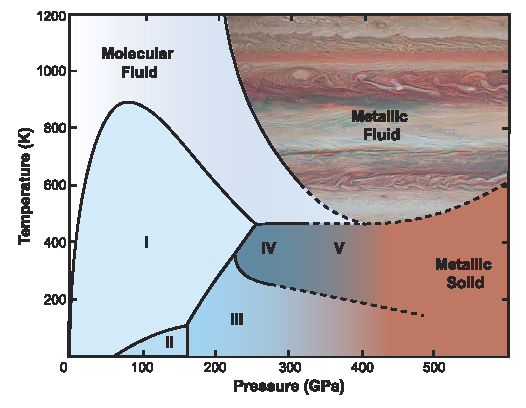
\includegraphics[width=0.49\textwidth]{phasediagram.pdf}
    \caption{The current phase diagram of dense hydrogen. The metallic fluid has been demonstrated in \cite{knudson2015} and is thought to make up the interiors of the Jovian planets \cite{ashcroft1968metallic}. The phases numbered I-V are the solid molecular phases of dense hydrogen. The metallic solid is coloured brown due to the theorised darkening of the metal due to bandgap closure. From \cite{gregoryanz2020}}
    \label{fig:phasediag}
\end{figure}
\vspace{3mm} %5mm vertical space


At pressures of 400--500 GPa and temperatures below about 450 K, hydrogen is predicted to transition to a metallic solid \cite{Wigner1935}. This material is of significant experimental interest as understanding the behaviour of the simplest element in extreme conditions can develop our understanding of fundamental interactions in condensed matter physics. Moreover, it is thought to display several fascinating properties including being a high-temperature superconductor \cite{ashcroft1968metallic}, meaning it could have a myriad of applications from low cost electricity distribution to efficient transport.

At temperatures above around 450 K and pressures around 300 GPa, hydrogen is a metallic fluid \cite{knudson2015}. Though this phase has also been of significant interest in recent years, especially in astrophysics as it is thought to make up the cores of the Jovian planets \cite{ashcroft1968metallic}, this paper will focus largely on the solid phase of MH.

The extreme pressures at which metallic hydrogen (MH) is thought to form means that making predictions about its properties, and making it in the lab, pose significant challenges. However, the potential benefits mean that there has been a concerted effort from both theorists and experimentalists to better understand this material and ultimately make it in the lab.

This paper aims to provide an overview of investigations into MH. Section \ref{sec:overview} will summarise current understanding of solid hydrogen and some of the main ideas about properties of MH. Section \ref{sec:model} will describe the challenges facing theorists making predictions about MH and the tools they are using. Finally, section \ref{sec:exp} will outline the experimental techniques used in attempts to make MH in the lab and some of the main challenges experimenters face when investigating this fascinating material will be discussed.


\vspace{7mm} %5mm vertical space

\section{High Pressure Hydrogen Physics: an Overview}
\label{sec:overview}
\vspace{2mm} %5mm vertical space

The properties of solid hydrogen up to 400 GPa below 450 K are well understood. In this region of the phase diagram, experimenters have observed five different phases (shown in figure \ref{fig:phasediag}), each characterised by a different arrangement of the lattice of \ce{H2} molecules.
%%%The first phase of dense hydrogen observed was phase I which exists up to about 900 K and 250 GPa \cite{mao1979}. The molecules are arranged in hexagonal close packed arrays and are freely rotating \cite{mao1994}. Phase II is formed by compressing phase I above 60 GPa below 100 K, and is known as the broken symmetry phase. This phase is dominated by quantum effects so details of the structure remain unknown, but diffraction evidence suggests that the structure may be at least partially ordered \cite{goncharenko_loubeyre_2005}. Phase III is obtained via further compression of phase I (below 350 K) or II \cite{hemley1988} and is thought to persist up to at least 400 GPa below 150 K. Compression of phase III at 330K causes a transition to phase IV at about 230 GPa \cite{Howie2012}, and continued compression at 200K up to 325 GPa causes a gradual transition to phase V. The most recently discovered phase, phase V is a semimetallic phase containing a mixture of the atomic and molecular structure \cite{dalladay2016} that is thought to be a precursor to the metallic phase. Even using the most modern analysis tools, only basic details of the structures of phases III-V are understood as at such high pressures, the quantum effects that dominate the lattice structures are extremely complex.

At pressures of 400--500 GPa below about 450 K, hydrogen is thought to metallise \cite{dalladay2016}. Under these conditions, the H-H bond is predicted to break so the structure becomes a lattice of H atoms, like in a metal. The bandgap (energy difference between the valence band---electrons involved in bonding---and the conduction band---electrons involved in conduction) will close as hydrogen changes from an insulator to a conducting metal \cite{Morales2013}. It is not known whether MH will be stable, but the most recent research suggests it will not persist in the metallic phase once the pressure is released \cite{ackland2017stability}.

Calculations using Bardeen, Cooper and Schrieffer (BCS) theory \cite{Solyom2009} suggest that electrons in MH should be able to form so called `Cooper pairs', boson like objects that carry current through the structure with no resistance, making it a superconductor. The critical temperature of MH is thought to be at least 300 K \cite{ashcroft1968metallic}. If this is correct, MH would be the world's first room temperature superconductor.

However, key details of the metallic phase (chiefly the precise conditions required for the transition) remain unknown as it is governed by complex interactions that make its properties extremely hard to predict.
%--------------------------------------------------------------------------
\vspace{7mm} %5mm vertical space
\section{Modelling Tools}
\label{sec:model}

%define better/clarify what's c2/c-24 ---> monserrat citation

\subsection{Structure Predictions in High-Density Hydrogen}

Predicting and studying the structural properties of high-density hydrogen is fundamental in understanding its distinctive behavior. The most relevant calculations have involved a structure named \textit{C2/c-24}. The \textit{C2/c-24} structure in solid hydrogen is a hexagon of mono-clinic symmetry, with 24 atoms of hydrogen per primitive cell \cite{Monserrat2016}, shown in Figure \ref{fig:crystal}. However, clear predictions are difficult because the extremely high pressures mean that the nuclei are packed very close, so the properties of MH are dominated by quantum nuclear effects---the effects of applying quantum dynamics to the nucleus of the particles \cite{loubeyre2020}. There have been many studies of possible structures of MH, leading to a multitude of propositions, each with their own complexities.

\begin{figure}[H]
\centering
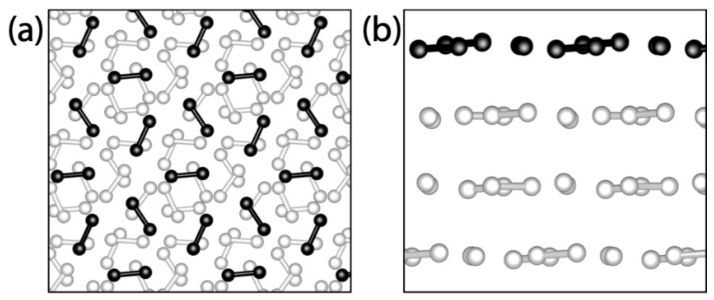
\includegraphics[width=0.49\textwidth]{cristal.png}
\caption{\label{fig:crystal}Proposed \textit{C2/c-24} crystal structure of MH at 400 GPa (a) top view and (b) side view. From \cite{Dogan2020}}
\end{figure}
\vspace{3mm} %5mm vertical space
An important property of MH that has been investigated using multiple different models is the closure of the bandgap. Figure \ref{fig:bandgap} shows how the bandgap is predicted to close under increasing pressure at 80 K using several different calculations with the \textit{C2/c-24} structure. The black rectangles and circles show the most recent experimental measurements of bandgap energy. While the models have some general agreement, there is significant variation due to different considerations in each model \cite{Morales2013}.

\begin{figure}[H]
\centering
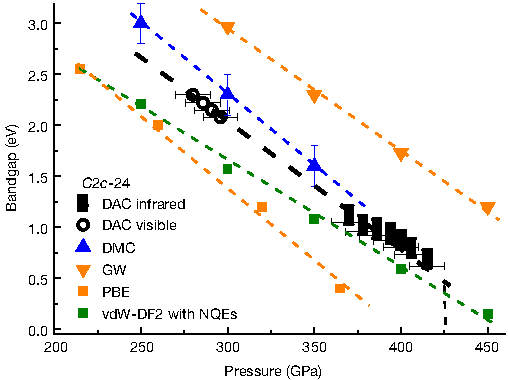
\includegraphics[width=0.49\textwidth]{bandgap.pdf}
\caption{\label{fig:bandgap} Variation of bandgap energy with pressure in solid Hydrogen at 80 K. The orange, green and blue data are predictions using different tools to model the \textit{C2/c-24} structure. The black rectangles and circles are recent experimental measurements from \cite{loubeyre2020} using a Diamond Anvil Cell (DAC).}
\end{figure}
\vspace{2mm} %5mm vertical space

\subsection{Modelling Tools}

\subsubsection*{Density Functional Theory (DFT)}

When attempting to predict the outcome of many interacting quantum particles, the problem is traditionally expressed as a 3N-dimensional Schrödinger equation. This involves setting up a 3-dimensional space including N particles resulting in a complicated Schrödinger equation for the wavefunction of the system. Density functional theory (DFT) recasts this problem into a density distribution (functional) of particles with a universal function of the density \cite{Gross2013}.

The main advantage of this method is that instead of solving a many-body Schrödinger equation, an approximation of the density functional can be used to solve the relevant single body Schrödinger equations, which are much simpler. The most popular approximation of the density functional is local density approximation (LDA). The ability of DFT to produce sufficiently accurate predictions using LDA without being overly computationally expensive has made DFT a popular modelling tool \cite{Gross2013}.

DFT can be improved upon by deriving better functionals (generally these are gradient corrections) \cite{Aryasetiawan1998}. One improved functional of DFT is the Perdew-Burke-Ernzerhof functional (PBE) which was used to predict the orange squares in figure \ref{fig:bandgap}  \cite{Bagayoko2014}.

Another improved functional is VDW-DF2 which accounts for the Van Der Waal’s (VDW) interactions between bodies in the system. Traditionally, in densely packed systems like solid hydrogen, VDW interactions are assumed to be negligible, but including these interactions improves predictions \cite{Lee2010} \cite{Berland2015}, as shown by the green squares in figure \ref{fig:bandgap}) which are closer to the experimental data than PBE.


\subsubsection*{Alternative Simulation Methods}
Alternatively, theorists can use tools other than DFT. A major weakness of DFT is that it does little to simulate the self-energy (impacts of a particle on itself and its environment) of the particles. 

The GW approximation, expresses the self-energy of a system in terms of a Green's function, G and the screened Coloumb interaction, W \cite{Aryasetiawan1998}. This produces significantly higher bandgap measurements (orange triangles in figure \ref{fig:bandgap}) than the other tools.

Another technique available is the Diffusion Monte-Carlo (DMC) simulation. Monte Carlo (MC) simulations use repeated random sampling to solve problems using a non-deterministic approach. This type of simulation uses random numbers to model complex systems and then returns a set of possible outcomes with different probabilities. DMC uses MC simulation to solve a many-body Schrödinger equation. However, this is extremely computationally expensive. To reduce this expense, DMC neglects the Nuclear Quantum Effects, which slightly reduces the accuracy of the simulation \cite{Markland2018}. DMC simulations were used to produce the blue line in figure \ref{fig:bandgap}. Of the tools available, it is in best agreement with the experimental results, but still slightly over-estimates the bandgap because quantum nuclear effects are neglected \cite{loubeyre2020}.

\subsection{Comparing Modelling Techniques}
Although several techniques have been applied to the problem of simulating hydrogen as a quantum solid, none have yet been able to make confident predictions about the MH transition. DMC and GW are generally considered more accurate than DFT as they do not rely on the approximations of the density functionals. However, DFT methods are adaptable and improvable, so developments are always being made. While DMC is in best agreement with the experimental results, the omission of nuclear quantum effects from the calculation means it slightly overestimates the bandgap.

With the addition of nuclear quantum effects, DMC has potential to improve further. Ultimately, precise simulations of MH remain beyond current capabilities. But with computing power constantly improving, firm predictions regarding the closure of the band-gap and the transition to solid MH may soon be available.

\vspace{7mm} %5mm vertical space
\section{Experimental Techniques}
\label{sec:exp}
%%%%%%%%%%%%%%%%%%%%%%%%%%%%%%%%%%
%Such pressures can readily be produced by 'dynamic pressure techniques' that produce a brief but extremely sharp rise in pressure. This is achieved via a projectile hitting the sample chamber with very high energy, causing a shock wave. Most success has been with multiple shock compression, where the initial shock wave reverberates between two anvils such that pressure increases in a series of steps until the final pressure is reached. A schematic of the apparatus for dynamic compression is shown in figure \ref{fig:dynamic_schem}. 

%of liquid hydrogen, inducing temperature and entropy that dissociates the bonds. This increase in pressure and temperature is 

Producing the extremely high pressures at which the transition to solid MH is predicted to occur poses a significant experimental challenge. The transition to liquid MH was first observed between 93--180 GPa by firing a projectile at a liquid sample at 3000 K \cite{weir1996}. However, this method cannot produce solid MH, as it only works for liquid samples. The pressure in the solid can be increased by crushing the sample between two pistons. However, the required pressures of 400--500 GPa break most materials so apparatus must be carefully constructed. The tool of choice for exploring dense hydrogen is the diamond anvil cell (DAC).

%A reverberating shock-wave compressed a thin 0.5mm layer of hydrogen to pressures of 93-180GPA and temperatures of 3000K. Electrodes attached to the sample measured a decrease in resistivity of four orders of magnitude that suggested the sample had transitioned to its superconducting fluid state. A schematic of the apparatus for dynamic compression is shown in figure \ref{fig:dynamic_schem}. Dynamic methods are not suited to produce solid MH however, as the method only works for liquid samples. Instead, "static pressure" techniques are needed to make the solid metallic phase. Static techniques involve the use of a "diamond anvil" to create high constant pressures of 400--500GPa at temperatures below 400K. These conditions are so extreme that most materials break before high enough pressures are generated. As such observing the transition to MH has proved extremely challenging.

%Most recently, dynamic techniques were used to observe the transition of liquid deuterium to a metallic fluid at temperatures around 1000K and pressures around 280 K, which helped determine the location of the phase transition between the molecular and metallic fluids shown in figure \ref{fig:phasediag} \cite{knudson2015}.

%However, dynamic methods are not appropriate for production of solid MH because the technique only works for liquid samples. Therefore, experimenters attempting to make the solid metallic phase use 'Static pressure' techniques. Static techniques usually involve crushing the sample between two pistons, but the pressures required for the transition to metal of 400--500 GPa below 450 are so high that most materials break before high enough pressures can be achieved. Producing high enough pressures to observe the transition to MH has therefore proved extremely challenging.

\subsection{Diamond Anvil Cell}

The DAC consists of two diamonds with their points facing each other. The diamonds can be pushed together, increasing the force and hence the pressure between the two tips. The sample is held between the tips in a gasket often made from Rhenium, and the pressure during compression is measured by continuous measurement of the properties of a material whose behaviour under pressure is well understood, such as ruby \cite{Burnley2018} or the diamond anvils themselves \cite{LoubeyreTDAC}. A schematic of the DAC is shown in figure \ref{fig:DACfig}.

When in the DAC, the sample can be illuminated by shining EM radiation through one of the diamonds so the sample can be studied using spectroscopic or diffraction techniques \cite{Burnley2018}. It is also possible to measure the electrical properties of the sample by attaching electrodes and measuring the resistance.

\begin{figure}[H]
    \centering
    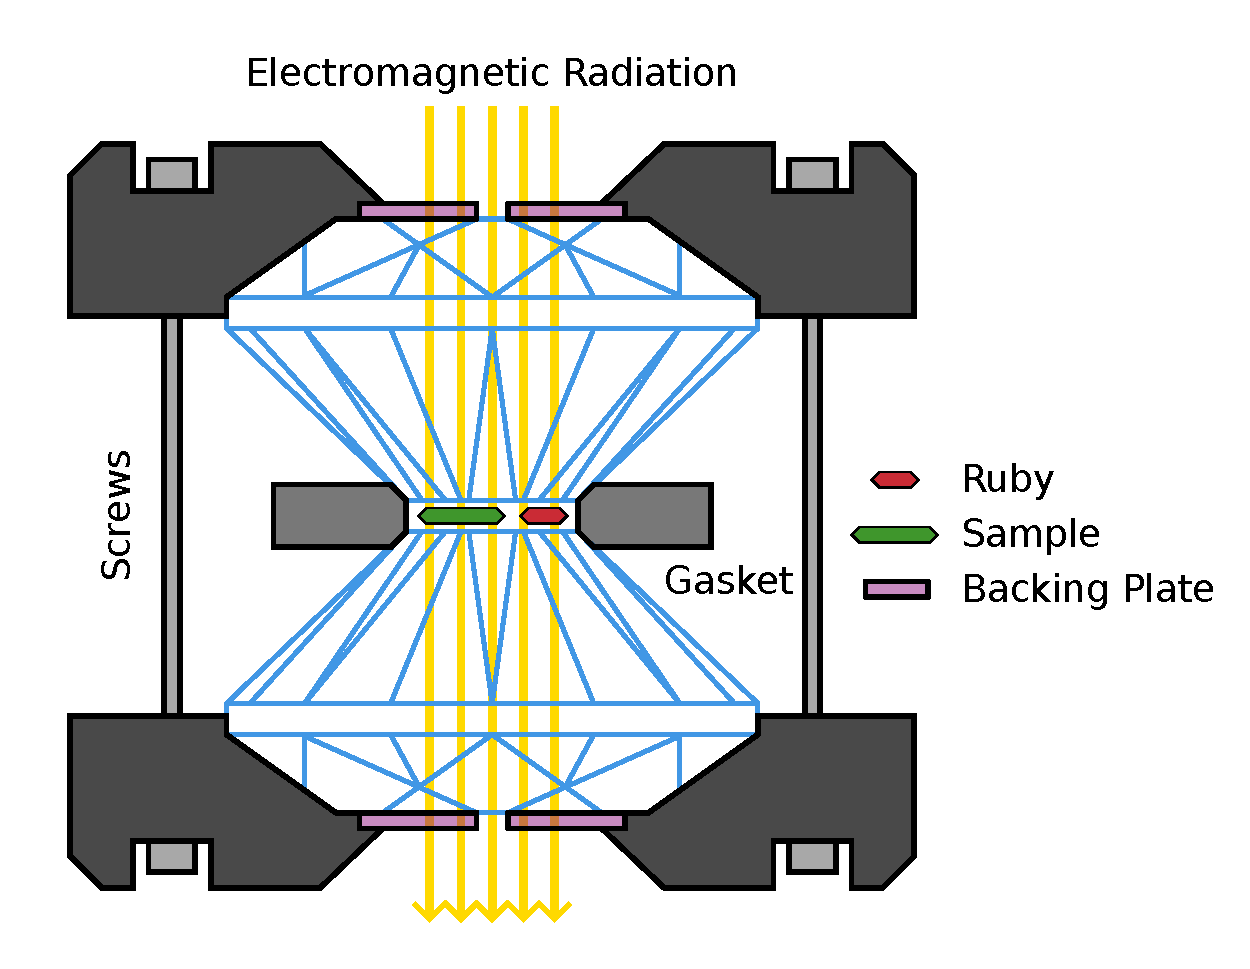
\includegraphics[width=0.49\textwidth]{DACfig.pdf}
    \caption{Schematic of a DAC. The gasket is typically around 100-250 microns in diameter. The pressure in the casket is increased by bringing the diamonds closer together. Pressure measurements use a reference material whose behaviour under pressure is well understood, like ruby. The sample is illuminated through the diamonds by EM radiation, allowing study by Raman spectroscopy or IS. Image from: \cite{tobias2012}}
    \label{fig:DACfig}
\end{figure}
\vspace{3mm} %5mm vertical space
However, the maximum pressure achievable in a conventional DAC is around 400 GPa, as at such pressures, even diamond begins to break \cite{li_ji_yang_2018}. Since metallisation is predicted around 400--500 GPa, it is unlikely that metallisation could be confirmed in an experiment using a conventional DAC as it will be difficult to verify the pressure measurement so close to the performance limit of the DAC.

In 2018, DAC performance was improved by shaping the diamond tips in a toroidal shape. The toroidal-DAC (T-DAC) is capable of producing pressures up to 1.5 times larger than standard DACs (up to 600 GPa) \cite{LoubeyreTDAC}, well beyond the predicted transition pressure. This technology has potential for making MH in the lab.

\subsection{Detecting the transition to metal}

Now that the predicted pressures for the transition to solid MH could be achievable in the lab, experimenters must turn their attention to verifying that the phase change has been observed. Detection of the predicted properties of MH: its structure, the closing bandgap, and superconductivity could provide good evidence that the transition has been observed.

\subsubsection{Measuring the structure of MH}

Since MH is predicted to have a \textit{C2-c24} structure \cite{Dogan2020}, detecting the formation of this structure could confirm creation of MH. Properties of lattices are usually investigated using X-ray diffraction (XRD) \cite{Nave2017XRD}. % The diffraction pattern produced when X-rays pass through a lattice depends on the lattice structure , so by analysing the diffraction pattern the lattice properties can be revealed.%
XRD is popular because X-ray sources are readily available and results can be produced quickly \cite{Dutrow2020}. XRD has been used to investigate MH in \cite{ji_li_liu_smith_et_al_2019} but a number of difficulties were reported. Chiefly, X-ray scattering power is proportional to the square of atomic number so hydrogen produces weak scattering. Moreover, several features of the lattice further weaken the signal and the DAC broke when illuminated by X-rays at high pressure.%Consequently, it took the researchers over five years to produce their results using extremely complicated techniques.

These difficulties make XRD impractical for investigations of dense hydrogen and have led researchers to pursue other techniques.

\subsubsection{Spectroscopic approaches}

Structural details can be revealed using spectroscopic techniques. The lattice structures of different phases of hydrogen vibrate in different ways, and these vibrations have certain allowed energy levels. Therefore, the different energy levels available to the lattice can provide information about the properties of hydrogen phases. For studying MH, the signal of the H-H bond is especially important, as it will break in the transition to MH. A weakening of the signal from this bond would imply the sample is metallising.

\begin{figure}[H]
\centering
\includegraphics[width=0.49\textwidth]{Loubeyre2a.pdf}
\caption{\label{fig:IR_Loubeyre} Possible IS evidence for the transition to MH given by relative absorbance (compared to at 123 GPa) of phase III at 80 K under increasing pressure. The point where absorbance goes to maximum gives the energy bandgap (shown by coloured arrows). At 427 GPa, absorbance is maximal over the whole range, showing the bandgap is lower than the IR energies used. The authors claim this shows the bandgap has closed because MH has formed \cite{loubeyre2020}.}
\end{figure}
\vspace{3mm} %5mm vertical space
Vibrational modes are investigated via infrared (IS) or Raman spectroscopy. In Raman spectroscopy, the sample is illuminated with monochromatic light in the visible, near-infrared, or near ultraviolet range. Some of the photon energy excites the molecules, so the photon energy changes as it passes through the lattice. The energy shifts reveal the transitions present in the molecule \cite{Nave2017Raman}. The first ever claim of solid hydrogen metallisation in 1989 used the loss of the Raman signal of the H-H bond in phase III hydrogen \cite{hemley1989}. However, further investigation  revealed the signal was lost because the sample was destroyed \cite{gregoryanz2020}.

In IS, the sample is illuminated by a range of infrared frequencies and photons with energy of modes available to the sample are absorbed. The absorption/transmission spectra reveal the modes that were present \cite{Brighthub}.

%By taking Raman or IR spectra of hydrogen samples in different conditions, such as by increasing the pressure, scientists can identify changes in the spectra that indicate structural changes due to phase transitions.%



%In spite of this setback, Raman spectroscopy has proven to be an extremely useful tool in investigations of dense hydrogen, with Raman spectra recently providing evidence of the existence of phases IV \cite{Howie2012}, and V \cite{dalladay2016}, and is likely to play a major role further investigations into the metallic state.

%%, and photons of frequencies not related to any modes will go through the sample. 

%%So, in the transmission spectra, the excitation modes of the hydrogen are observed and these can then be compared to other data or theoretical predictions to diagnose the phase and structure of the hydrogen.


\subsubsection{Closing bandgap}

Another feature of the energy levels that may reveal metallisation of hydrogen is bandgap closure. The most recent claim of MH made use of IS techniques to study this phenomenon \cite{loubeyre2020}. The spectra under increasing pressure are shown in figure \ref{fig:IR_Loubeyre}. The authors claim that the maximum absorbance across all wavelengths at 427 GPa shows the bandgap is zero because photons of all energies are absorbed. However, it is possible that the bandgap has simply fallen to an energy below the range investigated.

\begin{figure}[H]
    \centering
    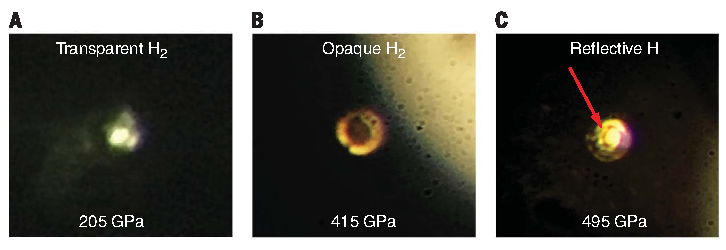
\includegraphics[width=0.49\textwidth]{DiasSilvera2017img.pdf}
    \caption{Microscope images of hydrogen sample under increasing pressure, taken with an iPhone. In each image, the slightly illuminated area around the sample (shown by the read arrow in C) is the casket holding the sample. The sample was illuminated from behind. A: below 325 GPa, the sample was transparent. B: above 325 GPa, closing bandgap caused transition to a semiconducting phase causing the sample to darken. C: The authors claim the high reflectivity of the sample at 495 GPa is caused by transition to MH \cite{dias_silvera_2017}.}
    \label{fig:DiasSilvera2017img}
\end{figure}
\vspace{3mm} %5mm vertical space
\subsubsection{Resistivity measurements}

Since metallic hydrogen is predicted to be a superconductor \cite{ashcroft1968metallic}, a drop in resistance of the sample would be strong evidence that it has transitioned to metal. However, electrodes can form metallic hydride upon contact with the sample, or the sample can be destroyed, making it easy to misinterpret results \cite{gregoryanz2020}.

\subsection{The Importance of Good Evidence}
%\subsection{Summary of techniques}
%%%%maybe not needed?
%To briefly summarise, the central techniques in diagnosing MH are: IS and RS which can be used in conjunction to probe excitation modes related to the phase of hydrogen, and resistivity measurements, where a sharp drop in resistance of the sample is associated with MH.

%MH can be observed with either dynamic or static pressure. Under dynamic pressure, LMH is observed at 140GPa and 3000K. These conditions are generated by impacting the chamber with a projectile, inducing shock waves which are then reverberated in the chamber. With static pressure, solid MH is thought to be produced at around 425GPa, 300K. The static pressures are generated via diamond anvil cells.


%Recent spectroscopic analysis in \cite{loubeyre2020} is perhaps the most convincing evidence yet of MH. However, no one has yet provided convincing resistivity measurements that would provide the strongest grounds to claim the transition to metalisation has occurred

Scientists are racing to confirm they have made MH in the lab, and such is the desire to be the first to make it that some scientists have begun to claim observation of MH even in the absence of convincing evidence.

For example, Dias and Silvera claimed ``An observation of the Wigner-Huntington transition to MH" \cite{dias_silvera_2017} in 2017. However, the main evidence in the paper was the photographs of the sample shown in figure \ref{fig:DiasSilvera2017img} which the authors claimed showed the sample becoming shiny when it metallises. However, they did not provide continuous measurements to confirm that the sample remained in the DAC and their pressure measurements were beyond the accepted limit of the DAC at the time so the scientific community was quick to dispute the paper \cite{goncharov2017comment,liu2017comment,eremets2017comments,loubeyre2017comment}.

Similarly, in 2011 Mikhail Eremets claimed transition to liquid MH using a combination of Raman and resistivity measurements \cite{eremets2011}. However, the weakening of the Raman signal of the H-H bond and fall in resistivity were later determined to be due to the sample being destroyed rather than the phase transition to the metal.

This highlights one of the big challenges when investigating the metallic phase. Many predictions rely on a physical quantity falling---such as the H-H spectroscopic signal being lost or the resistivity dropping. These features would also be observed if the sample were destroyed, so it is easy to produce false positives.\\

The most recent spectroscopic analysis in \cite{loubeyre2020} provides probably the best evidence to date of observing MH. But even in this paper, the authors themselves admit that without conclusive resistivity measurements, the claim remains disputed. Given the difficulty of making and detecting MH, a convincing claim will likely have to provide robust evidence from both spectroscopic and resistivity measurements to convince the scientific community that MH has been produced.

%In contrast, the public media tend to meet any claim of MH with great enthusiasm, perhaps due to an underlying desire to see MH made a reality. It is vital that the scientific community does not fall into the same trap. With so much interest, a claim that goes undisputed but turns out to be unfounded would be a disaster for the reputation of the scientific community. As such, the scientific community must remain vigilant to poorly evidenced claims and scientists claiming to have observed the transition must present indisputable evidence to back up their claims. With so many groups devoted to creating MH, it is only a matter of time until this evidence becomes available and MH becomes a reality.

%----------------------------------------------------------------------------

%\section{Recent Evolution and a Look Ahead}

%In recent years, improvements to high pressure tools, accompanied by developments in computing power allowing more accurate predictions of the properties of MH have brought scientists closer than ever to achieving the goal of producing MH in the lab. Standard DACs are limited to around 400 GPa\cite{LoubeyreTDAC} and so are unlikely to be capable of achieving pressures required to obtain MH. In 2018, an improvement was made by shaping the diamond tips in a toroidal shape which allows pressures 1.5 times larger than standard DACs (up to 600 GPa)\cite{LoubeyreTDAC}. These Toroidal Diamond Anvil Cells (T-DAC) have vastly improved experimental capabilities. The recent results from Loubeyre’s team made use of the T-DAC to produce energy measurements at extremely high pressures that were in excellent agreement with predictions based on recent DMC simulations. This provided perhaps the most convincing evidence of the transition to MH to date. However, without conductivity measurements, even these claims remain tentative \cite{loubeyre2020}.

%In his 2001 work summarising the status of modern physics, Nobel Laureate Vitaly Ginsburg listed high temperature and room temperature superconductivity and MH as two of the most important problems in physics \cite{ginzburg2001}.



%----------------------------------------------------------------------------
\vspace{10mm} %5mm vertical space
\section{Conclusions}
\vspace{3mm} %5mm vertical space
Making MH is considered one of the most important challenges in condensed matter physics. Understanding the properties of the simplest element in extreme conditions promises to provide a significant insight into fundamental phenomena. However, details of these properties remain extremely hard to predict due to strong quantum effects in closely packed hydrogen solids \cite{loubeyre2020}. Achieving it experimentally presents even more of a challenge due to the phenomenally high pressures required. New technology like the T-DAC is bringing experimenters a step closer to their goal, but the problem of confirming metallisation continues to be a significant challenge \cite{LoubeyreTDAC}. In particular, the extreme pressures can sometimes destroy the sample, resulting in a loss of the signal of the H-H bond and/or a drop in resistivity that can be mistaken for a transition to MH.

MH is predicted to be a room temperature superconductor and therefore has potentially revolutionary applications in many fields. However, given it is yet to be confirmed in the lab, potential applications remain years away. Moreover, current DAC techniques will only be capable of producing micrometer scale samples that are challenging to study in the lab, let alone use in industrial settings. In spite of these challenges, the potential for groundbreaking applications combined with the opportunity to improve understanding of fundamental principles in condensed matter physics, make it worth pursuing.


\vspace{10mm} %5mm vertical space

\vspace{5mm} %5mm vertical space

% Incluir las referencias
%\insertbibliography{Referencias.bib}
\line(1,0){225}

\printbibliography


\line(1,0){225}

\end{document}
